\section{Intrinsic signal optical imaging settings}
\label{sec:Intrinsic-signal-optical-imaging-settings}

The course of action with each craniotomized mouse started with the performance of intrinsic signal optical imaging (ISOI) over the mice's primary visual cortex and surrounding visual areas [REFERENCES] to obtain a reasonable spatial resolution retinotopic mapping of the temporaly dependent hemodynamics of the accessed brain while moving visual stimuli was presented to the animal on a monitor aligned to the center of the mouse's right eye and forming a $30º$ angle with the animal's nose-line.

The stimuli consisted of a checkerboard of alternate flickering light/dark squares ($5 Hz$) that was masked to continuously expose only a periodic drifting stripe of the grid in four consecutive cardinal directions ($12 s$ period, $20º$ width, 80 times for each direction) - an horizontal stripe going from the top to the bottom of the screen, vice-versa, a vertical stripe going from its left to its right or in the opposite direction.[GET IMAGE]

The cortical surface of an head-fixed mouse was illuminated with a $620 nm$ red LED to allow the intrinsic hemodynamic signals to be recorded as optical images of reflectance change correspondent to cortical activity. This recording was held using a Retiga QIClick camera (QImaging) controlled with Ephus[REFERENCE] with a high magnification zoom lens (Thorlabs) at $5 Hz$ focused under the cranial window, at the brain surface. A $535 nm$ green LED was also used to obtain an image of the cortical vasculature.

For each animal, this resulted in a retinotopical map of $512 \times 512$ pixels, representing $?? \times ??$ of cortical area. This corresponded to the color-map of cortical encoding of both azimuth and elevation stimuli locations, superimposed on the image of the mouse's vasculature (images \ref{vessels} and \ref{mapping}). These correspondence figures were subsequently used as a first-approach guide to encountering the V1 positions aimed for imaging - those whose neurons responded to stimuli in the center of the mouse's visual field where the central stimuli were displayed during the following two-photon microscopy imaging sessions.

\begin{figure}[H] \centering 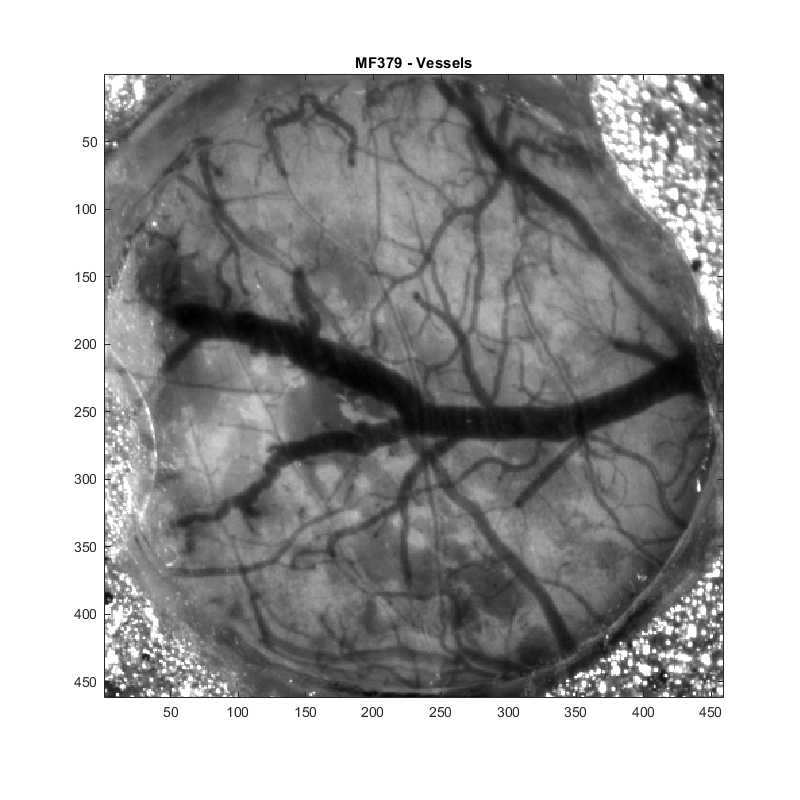
\includegraphics[width=7cm,height=7cm,keepaspectratio]{Figures/7.Results/intrinsic/MF379_Vessels.png} 
\caption{animal by Marina.}
\label{vessels}

\end{figure}

\begin{figure}[H] \centering 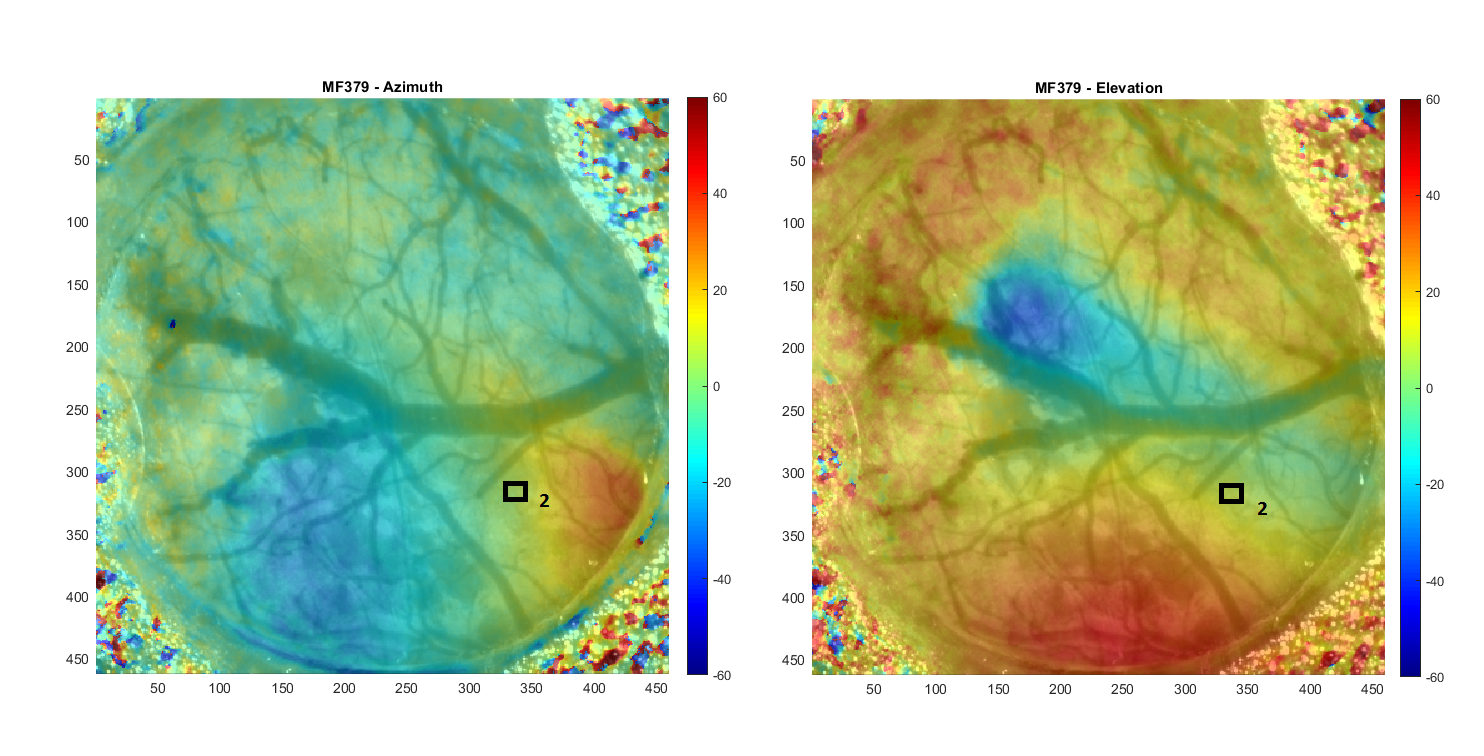
\includegraphics[width=13cm,height=13cm,keepaspectratio]{Figures/7.Results/intrinsic/mapping.png} 
\caption{animal by Marina.}
\label{mapping}
\end{figure}

%\subsection{Subsection A}
%\label{subsec:subasectionA}